\chapter{Design}

% Can be inconsistent with implementation but make sure you give reasons
% Choice of library and use case diagram

\section{Experiments}

Due to the time constraints, each experiment will run for six days. As cress is a fast growing herb, this should be sufficient time for the environment to have enough of an effect to show in its growth. The seventh day will then be used to take measurements of all the cress, clean the greenhouse and alter the code to create the next new growing conditions.

Although cress can be grown using hydroponics, the greenhouse will contain soil to keep the cress seeds in place. This also makes it easier to measure the moisture level as the moisture sensor can be placed in the soil and not straight into water which will continue to measure the same value. This soil will not be entirely changed for each round, instead topped up when necessary in order to maintain the same weight throughout each round. However, the water will be drained, cleaned and replaced to prevent growths, algae or mould appearing in the greenhouse and prevent it from getting caught in the water pump.

To keep all the experiments fair, they will all be using the same number of cress seeds. As the cress will be measured manually after the growing period, there shouldn't be an unreasonable amount, this also gives the cress space to grow and not interfere with each other. With space surrounding each seed, given the small space of the greenhouse, I plan to use 12 cress seeds per round of the experiment.

The measurements taken by hand will be measure with a ruler and stored in an excel spreadsheet. All the measurements taken by the greenhouse will be stored in a CSV file. These two files will then be joined and used to create the graphs for evaluation and to make a final conclusion on the project.

The experiments to run are as follows:

\begin{center}
\begin{tabular}{| c | c | c | c | c | c | c |} 
    \hline
    \textbf{Light} & White & No light & Red & Blue & White & White\\
    \hline
    \textbf{Moisture(v)} & 0.5 & 0.5 & 0.5 & 0.5 & 1 & 2\\
    \hline
\end{tabular}
\end{center}

The first experiment will be the control and will consist of a white light at maximum brightness with a constant moisture level of 0.5v. This will be used as a control run and all the other experiments will be compared to it to find which variables are affecting the growth in certain ways.

The following experiments change either the light colours or the moisture level. Experiments 2 - 4 maintain the same moisture level as the control but change the colour of the light. Experiments 5 and 6 maintain the same white light but with varying moisture levels. Using these experiments, we can see how water and light can affect the growth of the cress.

\subsection{Hypothesis}

An article written about how different light qualities and intensities affect the growth and volatile compounds in plants state how their experiments conclude with higher light intensity resulting in increase of “root length, and leaf, shoot, root, and total weight” \cite{bayir2019plant}. It also concluded with red light showing highest leaf and total dry weight alongside a reduction in total monoterpenes, which are naturally occurring fragrant molecules with over 400 different structures \cite{ALCANTARA2011309}. Comparing this to blue light which showed a higher production in carvacrol which is a monoterpene often found in many aromatic plants used as spices such as oregano \cite{bayir2019plant}.

This leads to my hypothesis being that the control experiment with highest intensity of white light will have the longest stems and roots and therefore overall mass. Out of all the monochromatic lights, we will see if the red LED leads to the largest leaf span compared to the other colours. Unfortunately, I am unable to obtain the necessary equipment to measure the levels of different monoterpenes in the cress. For this reason, I will still be running an experiment with blue light, not to measure the monoterpene levels, but to compare the leaf length and other components to the white and red light experiments.

\section{Library}

\subsection{Design Pattern}
To deal with the number of different peripherals, I will be using the design pattern Facade. This is a structural design pattern that provides an interface to the library \cite{designPatterns}. The interface will hide the complexity and make creating experiments simple for beginners yet flexible enough for more confident users.

\begin{figure}[ht]
    \centering
    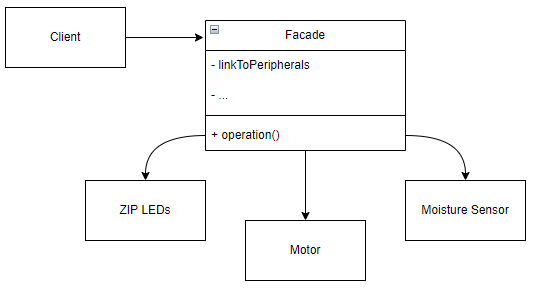
\includegraphics{Report/Images/facadePattern.png}
    \caption{Simplified class diagram using a facade design pattern}
    \label{fig:classDiagram}
\end{figure}

The advantage of using a facade design pattern is that we can improve the usability of the library for the user.  However we want to avoid coupling the interface with too many classes. Often times, the main facade class can be linked with an additional facade to control other classes in the subsystem. \cite{designPatterns}

All the hardware that the greenhouse makes use of have their own class. These classes are then nested inside the facade class so that it can be used as an interface. This also allows the code to be extended without too much difficulty for new hardware and future refactorings. Having all these classes nested also allows the users to be able to just import one library and have control over all the hardware needed for the greenhouse together without having a list of imports.

Each hardware component will have its corresponding class which will contain all the methods necessary to control it. For example, the class representing the zip LED will contain methods to change the colour of each LED and turn them on in any permutation the user wishes. The motor for the water pump may be turned on and off directly, or may be on for a specified time in seconds before being turned off automatically.

The concrete creator class instantiates an instance of the facade class which is the interface to the library. The concrete creator class encapsulates the creation of an instance. This approach promotes modularity and flexibility as changes to the concrete product can be isolated from the concrete creator class and the client code.
